% Mechanism diagram for "Observational uncertainty dominates climate impact projections"
% Standalone TikZ figure (tight bounding box). Compile with:
%   pdflatex extdata_fig3_mechanism.tex
%
% Three-colour palette:
%   slate      -> data inputs           (top decision, GCM ensemble)
%   blue       -> analysis              (Analyst-side card, bias-correct & downscale, amplification)
%   terracotta -> calculated values     (fitted D(T), future climate at GWL, projected impact)
\documentclass[tikz, border=3mm, 10pt]{standalone}
\usepackage[T1]{fontenc}
\usepackage{lmodern}
\usepackage{xcolor}
\usepackage{amsmath,amssymb}
\usetikzlibrary{positioning, arrows.meta, calc, fit, backgrounds}
% Suppress hyphenation throughout (narrow columns break ugly otherwise)
\hyphenpenalty=10000\exhyphenpenalty=10000

% ---------- 3-role palette ----------
\definecolor{datac}{HTML}{475569}      % slate      -> data input
\definecolor{dataLt}{HTML}{E2E8F0}
\definecolor{choicec}{HTML}{1D4ED8}    % blue       -> analysis
\definecolor{choiceLt}{HTML}{DBEAFE}
\definecolor{derivedc}{HTML}{B85042}   % terracotta -> calculated value
\definecolor{derivedLt}{HTML}{FBE7E1}
\definecolor{inkc}{HTML}{1F2937}
\definecolor{mutedc}{HTML}{6B7280}

% ---------- bullet macro for the Analyst card ----------
% Label in bold, why-it-matters inline as smaller italic muted text.
\newcommand{\bulC}[2]{%
  \textcolor{choicec}{\rule[0.3ex]{1.6mm}{1.6mm}}\,\textbf{#1}\,%
  {\scriptsize\itshape\textcolor{mutedc}{#2}}\par\vspace{2pt}}

% ---------- tikz styles ----------
\tikzset{
  topnode/.style    ={rectangle, rounded corners=2pt, fill=datac, text=white,
                      inner sep=5pt, align=center, font=\sffamily\small},
  choiceCard/.style ={rectangle, rounded corners=2pt, fill=choiceLt, draw=choicec,
                      line width=0.4pt, inner xsep=4pt, inner ysep=5pt,
                      align=left, font=\sffamily\footnotesize, text=inkc},
  dataNode/.style   ={rectangle, rounded corners=2pt, fill=datac, text=white,
                      inner sep=4pt, align=center, font=\sffamily\footnotesize},
  choiceNode/.style ={rectangle, rounded corners=2pt, fill=choiceLt, draw=choicec,
                      line width=0.4pt, inner sep=4pt, align=center,
                      font=\sffamily\footnotesize, text=inkc},
  derivedNode/.style={rectangle, rounded corners=2pt, fill=derivedLt, draw=derivedc,
                      line width=0.5pt, inner sep=4pt, align=center,
                      font=\sffamily\small, text=inkc},
  % "Amplification" box: same role/colour as analysis (blue), but left-aligned
  % because its body is a longer sentence.
  ampNode/.style    ={rectangle, rounded corners=2pt, fill=choiceLt, draw=choicec,
                      line width=0.5pt, inner sep=4pt, align=left,
                      font=\sffamily\footnotesize, text=inkc},
  % Terminal node: filled terracotta (calculated value) with white text.
  termNode/.style   ={rectangle, rounded corners=2pt, fill=derivedc, text=white,
                      inner sep=5pt, align=center, font=\sffamily\small},
  flow/.style       ={-{Stealth[scale=0.9]}, line width=0.5pt, color=inkc},
  flowdash/.style   ={-{Stealth[scale=0.9]}, line width=0.5pt, dashed, color=inkc},
}

\begin{document}
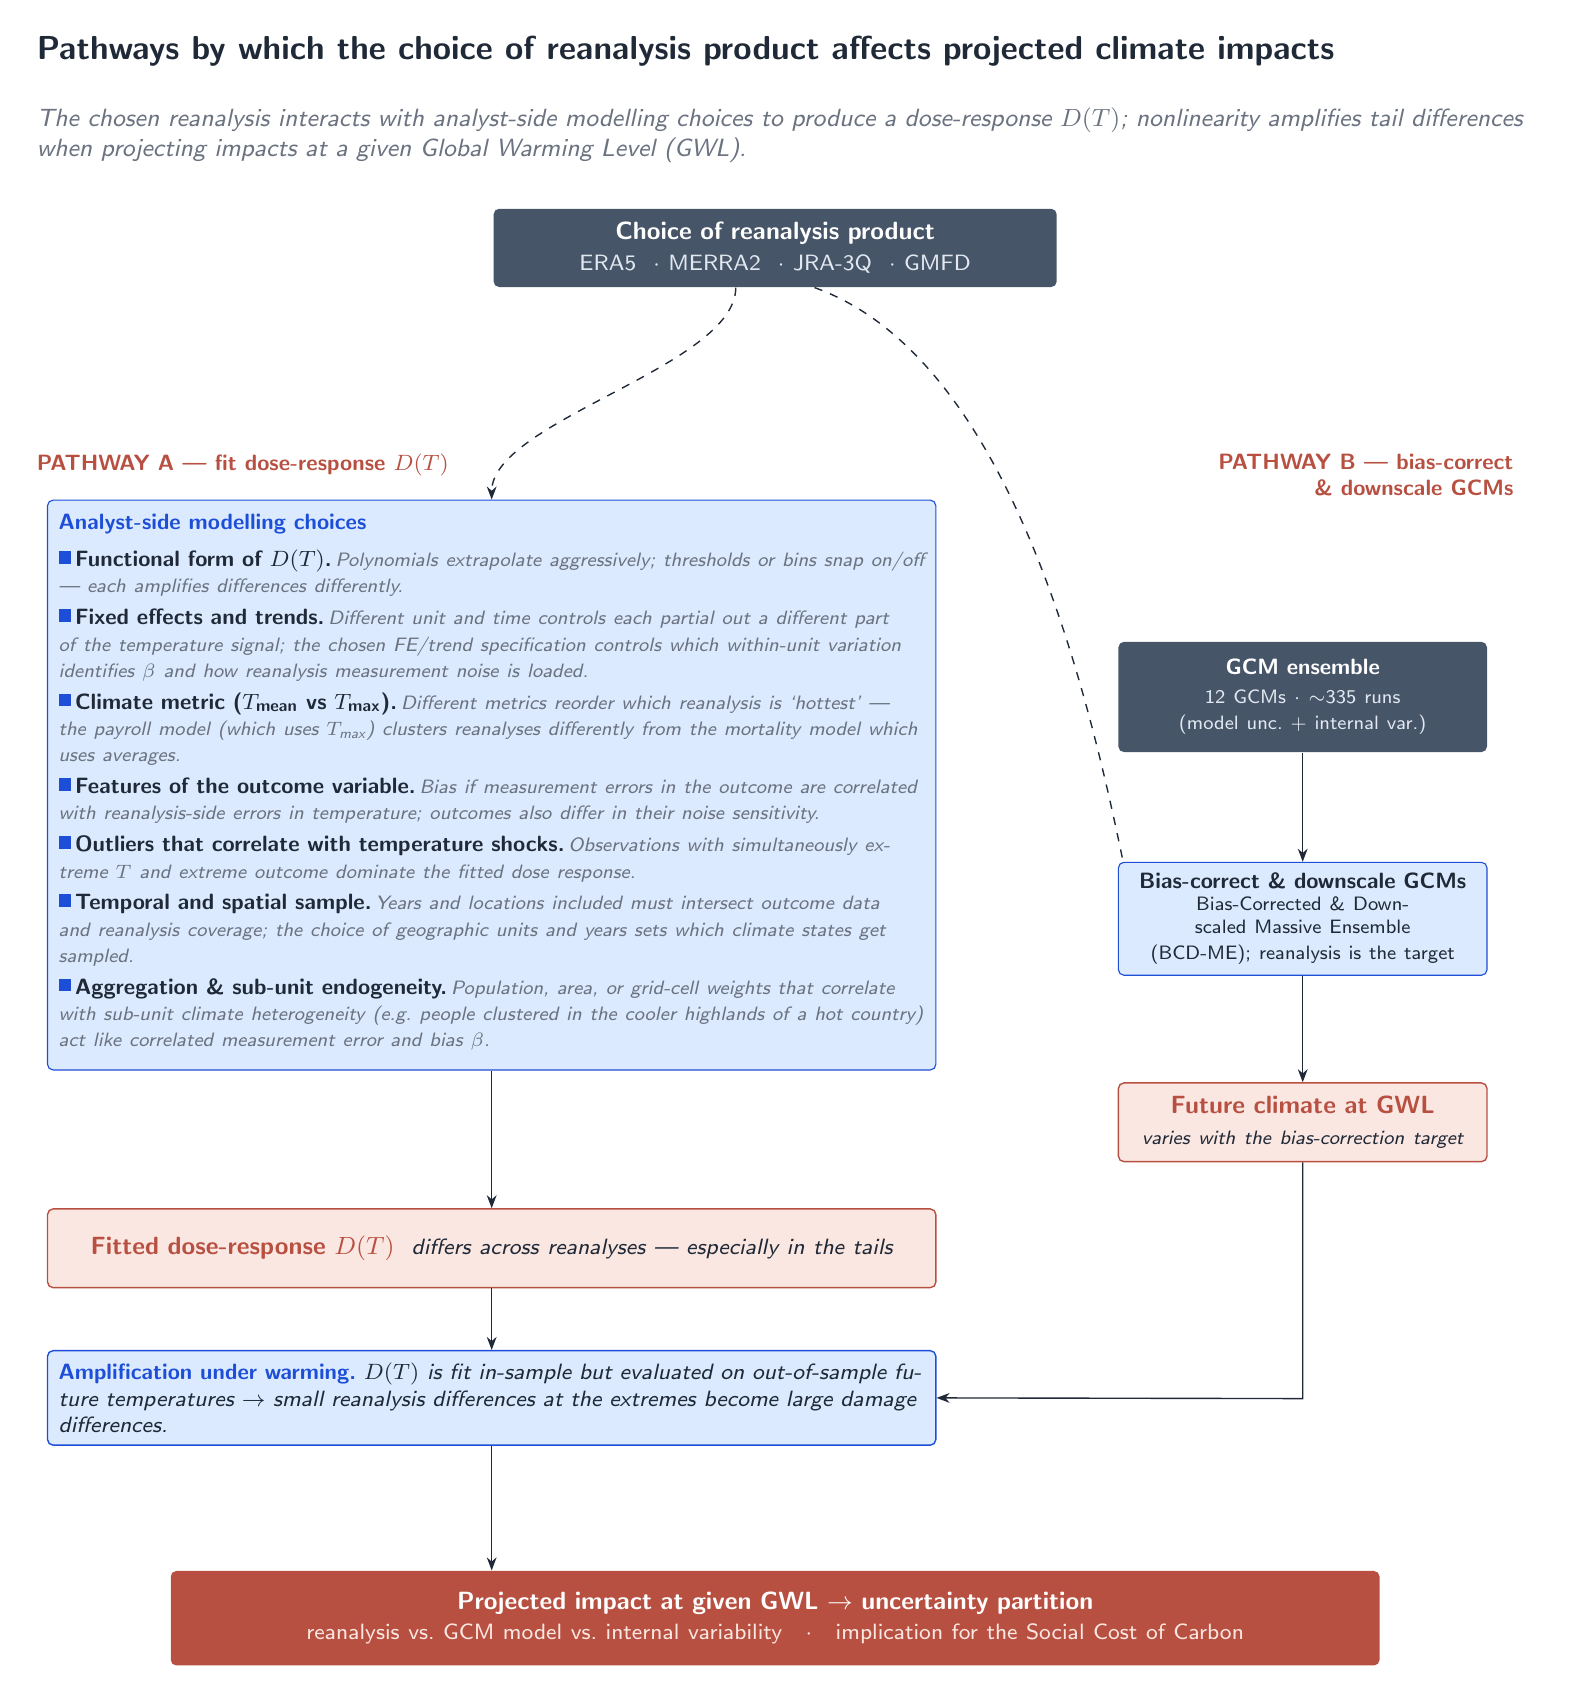
\begin{tikzpicture}[x=1mm, y=-1mm]

% ============================================================
% Title and subtitle
% ============================================================
\node[anchor=north west, font=\sffamily\bfseries\large, text=inkc, text width=190mm]
  at (0, 0)
  {Pathways by which the choice of reanalysis product affects projected climate impacts};

\node[anchor=north west, font=\sffamily\itshape\small, text=mutedc, text width=190mm]
  at (0, 9)
  {The chosen reanalysis interacts with analyst-side modelling choices to produce a
   dose-response $D(T)$; nonlinearity amplifies tail differences when projecting impacts at
   a given Global Warming Level (GWL).};

% ============================================================
% Top decision node
% ============================================================
\node[topnode, anchor=north, text width=68mm] (top) at (95, 23)
  {\textbf{Choice of reanalysis product}\\
   {\footnotesize\textcolor{dataLt}{ERA5 \ $\cdot$\ MERRA2 \ $\cdot$\ JRA-3Q \ $\cdot$\ GMFD}}};

% ============================================================
% Pathway labels
% ============================================================
\node[anchor=north west, font=\sffamily\bfseries\footnotesize, text=derivedc]
  (Alabel) at (0, 53) {PATHWAY A --- fit dose-response $D(T)$};

\node[anchor=north east, font=\sffamily\bfseries\footnotesize, text=derivedc,
      text width=42mm, align=right]
  (Blabel) at (190, 53) {PATHWAY B --- bias-correct\\\& downscale GCMs};

% Dashed branching arrows: reanalysis choice enters BOTH pathways.
\draw[flowdash] ($(top.south)+(-5,0)$) .. controls +(0,10) and +(0,-10) .. (59, 60);
\draw[flowdash] ($(top.south)+(5,0)$)  .. controls (125,42) and (135,85) .. (140, 110);

% ============================================================
% PATHWAY A: single (widened) Analyst-side modelling-choices card
% ============================================================
\node[choiceCard, anchor=north, text width=110mm] (choices)
  at (59, 60) {%
  \textbf{\textcolor{choicec}{Analyst-side modelling choices}}\par\vspace{4pt}
  \bulC{Functional form of $D(T)$.}%
       {Polynomials extrapolate aggressively; thresholds or bins snap on/off --- each amplifies differences differently.}
  \bulC{Fixed effects and trends.}%
       {Different unit and time controls each partial out a different part of the temperature signal; the chosen FE/trend specification controls which within-unit variation identifies $\beta$ and how reanalysis measurement noise is loaded.}
  \bulC{Climate metric ($T_\text{mean}$ vs $T_\text{max}$).}%
       {Different metrics reorder which reanalysis is `hottest' --- the payroll model (which uses $T_\text{max}$) clusters reanalyses differently from the mortality model which uses averages.}
  \bulC{Features of the outcome variable.}%
       {Bias if measurement errors in the outcome are correlated with reanalysis-side errors in temperature; outcomes also differ in their noise sensitivity.}
  \bulC{Outliers that correlate with temperature shocks.}%
       {Observations with simultaneously extreme $T$ and extreme outcome dominate the fitted dose response.}
  \bulC{Temporal and spatial sample.}%
       {Years and locations included must intersect outcome data and reanalysis coverage; the choice of geographic units and years sets which climate states get sampled.}
  \bulC{Aggregation \& sub-unit endogeneity.}%
       {Population, area, or grid-cell weights that correlate with sub-unit climate heterogeneity (e.g.\ people clustered in the cooler highlands of a hot country) act like correlated measurement error and bias $\beta$.}};

% ============================================================
% PATHWAY B: vertical chain on the right
% ============================================================
\node[dataNode, anchor=north, text width=44mm, minimum height=14mm] (gcm)
  at (162, 78)
  {\textbf{GCM ensemble}\\[1pt]
   {\scriptsize\textcolor{dataLt}{12 GCMs $\cdot$ $\sim$335 runs}}\\
   {\scriptsize\textcolor{dataLt}{(model unc.\ + internal var.)}}};

\node[choiceNode, anchor=north, text width=44mm, minimum height=12mm] (bcd)
  at (162, 106)
  {\textbf{Bias-correct \& downscale GCMs}\\
   {\scriptsize Bias-Corrected \& Downscaled Massive Ensemble\\(BCD-ME); reanalysis is the target}};

\node[derivedNode, anchor=north, text width=44mm, minimum height=10mm] (fut)
  at (162, 134)
  {\textbf{\textcolor{derivedc}{Future climate at GWL}}\\
   {\scriptsize\itshape varies with the bias-correction target}};

\draw[flow] (gcm.south) -- (bcd.north);
\draw[flow] (bcd.south) -- (fut.north);

% ============================================================
% D(T)  ->  Amplification  ->  Terminal
% ============================================================
\node[derivedNode, anchor=north, text width=110mm, minimum height=10mm] (dt)
  at (59, 150)
  {\textbf{\textcolor{derivedc}{Fitted dose-response $D(T)$}}~~%
   \footnotesize\itshape differs across reanalyses --- especially in the tails};

% Single arrow from the (now sole) Analyst card down to D(T).
\draw[flow] (choices.south) -- (dt.north);

\node[ampNode, anchor=north, text width=110mm, minimum height=12mm] (amp)
  at (59, 168)
  {\textbf{\textcolor{choicec}{Amplification under warming.}}\ %
   \footnotesize\itshape $D(T)$ is fit in-sample but evaluated on out-of-sample future
   temperatures $\to$ small reanalysis differences at the extremes become large damage
   differences.};

\draw[flow] (dt.south) -- (amp.north);

\node[termNode, anchor=north, text width=150mm, minimum height=12mm] (term)
  at (95, 196)
  {\textbf{Projected impact at given GWL $\to$ uncertainty partition}\\
   {\footnotesize\textcolor{derivedLt}{reanalysis~vs.~GCM model~vs.~internal variability\quad$\cdot$\quad implication for the Social Cost of Carbon}}};

% Future climate is *applied to* D(T): route into the Amplification box from the
% right (L-shape), making the multiplicative interaction visible.
\draw[flow] (fut.south) -- ($(fut.south)+(0,30)$) -- (amp.east);
% Combined result flows from Amplification down to the terminal.
\draw[flow] (amp.south) -- (amp.south |- term.north);

\end{tikzpicture}
\end{document}
